\documentclass[12pt]{article}\usepackage[]{graphicx}\usepackage[]{color}
% maxwidth is the original width if it is less than linewidth
% otherwise use linewidth (to make sure the graphics do not exceed the margin)
\makeatletter
\def\maxwidth{ %
  \ifdim\Gin@nat@width>\linewidth
    \linewidth
  \else
    \Gin@nat@width
  \fi
}
\makeatother

\definecolor{fgcolor}{rgb}{0.345, 0.345, 0.345}
\newcommand{\hlnum}[1]{\textcolor[rgb]{0.686,0.059,0.569}{#1}}%
\newcommand{\hlstr}[1]{\textcolor[rgb]{0.192,0.494,0.8}{#1}}%
\newcommand{\hlcom}[1]{\textcolor[rgb]{0.678,0.584,0.686}{\textit{#1}}}%
\newcommand{\hlopt}[1]{\textcolor[rgb]{0,0,0}{#1}}%
\newcommand{\hlstd}[1]{\textcolor[rgb]{0.345,0.345,0.345}{#1}}%
\newcommand{\hlkwa}[1]{\textcolor[rgb]{0.161,0.373,0.58}{\textbf{#1}}}%
\newcommand{\hlkwb}[1]{\textcolor[rgb]{0.69,0.353,0.396}{#1}}%
\newcommand{\hlkwc}[1]{\textcolor[rgb]{0.333,0.667,0.333}{#1}}%
\newcommand{\hlkwd}[1]{\textcolor[rgb]{0.737,0.353,0.396}{\textbf{#1}}}%
\let\hlipl\hlkwb

\usepackage{framed}
\makeatletter
\newenvironment{kframe}{%
 \def\at@end@of@kframe{}%
 \ifinner\ifhmode%
  \def\at@end@of@kframe{\end{minipage}}%
  \begin{minipage}{\columnwidth}%
 \fi\fi%
 \def\FrameCommand##1{\hskip\@totalleftmargin \hskip-\fboxsep
 \colorbox{shadecolor}{##1}\hskip-\fboxsep
     % There is no \\@totalrightmargin, so:
     \hskip-\linewidth \hskip-\@totalleftmargin \hskip\columnwidth}%
 \MakeFramed {\advance\hsize-\width
   \@totalleftmargin\z@ \linewidth\hsize
   \@setminipage}}%
 {\par\unskip\endMakeFramed%
 \at@end@of@kframe}
\makeatother

\definecolor{shadecolor}{rgb}{.97, .97, .97}
\definecolor{messagecolor}{rgb}{0, 0, 0}
\definecolor{warningcolor}{rgb}{1, 0, 1}
\definecolor{errorcolor}{rgb}{1, 0, 0}
\newenvironment{knitrout}{}{} % an empty environment to be redefined in TeX

\usepackage{alltt}
\usepackage[top=1.00in, bottom=1.0in, left=1.1in, right=1.1in]{geometry}
\renewcommand{\baselinestretch}{1.1}
\usepackage{graphicx}
\usepackage{natbib}
\usepackage{amsmath}
\bibliographystyle{..//refs/styles/besjournals.bst}
\def\labelitemi{--}
\parindent=24pt
\usepackage{lineno}
\linenumbers


\title{Reconciling competing hypotheses regarding flower-leaf sequences in temperate forests for fundamental and global change biology}

\author{Daniel Buonaiuto, Nacho, Lizzie}
\date{September 25, 2019}
\IfFileExists{upquote.sty}{\usepackage{upquote}}{}
\begin{document}

\maketitle

\begin{enumerate}
\end{enumerate}
\section*{Abstract}
\indent\indent It is not only individual phenological events that affect organism fitness, but also the relationship between events. Deciduous woody plants exhibit considerable variation in the relative order of their reproductive and vegetative events, or their flower-leaf sequence (FLS). Research suggests that FLSs are adaptive, and several competing hypotheses may explain their function. Reconciling these hypotheses has been impeded by our conceptual orientation towards them. Classically, FLSs are treated as discrete categories at the species level, obscuring important inter-specific differences and ignoring substantial intra-specific variation. Here, we develop the existing hypotheses to account for the inter- and intra-specific FLS variation seen in nature and evaluate these hypotheses with four case studies. Our inquiry provides three major insights towards a new framework for understanding FLSs. First, we find concurrent support for multiple hypotheses. Future research should allow for overlapping hypotheses and test individual hypotheses in smaller sub-groupings. Second, support for FLS hypotheses is highly sensitive to how FLSs are defined. Researchers should move away from categorization and use continuous measures of FLS. Finally, researchers should use an intra-specific approach to evaluate fitness consequences of FLS variation to help predict how climate-related alterations to FLSs will affect plant communities.\\


% ...to reduce the impact of observer bias, and allow for stronger inference regarding FLS variability among and within species
%Am nat 200 words
%250 AJB
%350 JoE
%currently 297


\section*{Introduction}
% Good stuff here in the first couple paragraphs
\indent \indent Phenology, the timing of seasonal life cycle events, allows organisms to synchronize important life history transitions with optimum environmental conditions \citep{Forrest2010}, and is a critical component of ecosystem structure and function \citep{Cleland2007,Piao2007}. Recent work in woody plant phenology has shown that it is not only individual phenological stages that affect these processes, but also the relationships between them \citep{Ettinger2018}.\\
\indent One phenological relationship that has long received scientific interest \citep[see][]{Robertson1895}, and recently, increased attention in the literature \citep{Savage2019, Gougherty2018} is the flower-leaf phenological sequence (FLS) of deciduous woody plants. In a typical model of plant life-history, vegetative growth precedes reproduction. However, for many species in the forests of Eastern North America, it is not the green tips of new shoots that mark the commencement of the growing season, but the subtle reds and yellows of their flowers. This flowering-first FLS is common in these regions, and its prevalence suggests that this FLS has adaptive significance \citep{Rathcke_1985}.\\ 

\indent A deep inquiry into the nature of this phenological pattern is necessary and particularly timely now because anthropogenic climate change is altering FLSs (Fig. \ref{fig:Figure 1}). For the three European tree species we examined, the number of days between flowering and leafout have increased as a result of climate change, but the rate of change differs among them. If, as suggested, optimum not FLS patterning is an important component of fitness, this differential FLS sensitivity to climate change may influence which species will persist under altered climate conditions.\\

\indent Despite recent advances in characterizing the evolution and underlying physiology of FLS \citep{Gougherty2018,Savage2019}, a major challenge to predicting how FLS patterns will shift in response to climate change is that we do not have a solid baseline understanding of variability in FLS. While some authors present general correlations between flowering and leafing phenology \citep{Lechowicz_1995, Ettinger2018}, fine-scale FLS variability has never been evaluated. We suggest that characterizing FLS variation among individuals and populations will not only improve our ability to predict how FLS patterns will change in the future, but also allow for a more biologically relevant evaluation of the current FLS hypotheses, revealing avenues for future, direct hypothesis testing.\\

\indent Here we 1) Review the hypotheses of woody plant FLSs and their respective predictions, 2) Evaluate variation in FLSs, and explore how FLS variation within species, populations and individuals alters the predictions of the hypotheses, 3) Show how the incorporation of variation reveals consistencies and anomalies in support for FLS hypotheses using several case studies from temperate forests, and 4) make recommendations for future study of FLSs. 

\section*{Defining FLS}

\indent\indent Flower-leaf sequences have traditionally been classified into qualitative categories that are almost always defined at the species level. The terms hysteranthy, protanthy, proteranthy or precocious flowering describe plants that produce flowers before their leaves. Synanthy describes species whose flowering period overlaps their leaf development and seranthy describes plants whose flowers open after their leaves emerge \citep{Lamont2011, Heinig1899}. But applying these conceptual categories to real phenological sequences is not always so straight forward.\\

\indent Both reproductive and vegetative phenological sequences consist of multiple sub-stages, and this introduces significant ambiguity into how we interpret qualitative FLS descriptions. Consider a species with the following FLS:\\
\begin{center}
\textbf{flower budburst}\rightarrow \textbf{leaf budburst}\rightarrow \textbf{first flowers open} \rightarrow \textbf{leafout} \rightarrow \textbf{peak flowering} \rightarrow \textbf{end of leaf expansion}\\
\end{center}

\indent Phenological observers might classify this species as hysteranthous because flower budburst proceeds leaf budburst. They would also be justified if they called this species synanthous because flowers open during the time between leaf budburst and leafout. But they could just as easily categorize this species as seranthous because peak flowering occurs after leafout.We can see that in the long term phenologiical records from Harvard Forest in Petersham, MA \citep{OKeefe2015} that the same ambiguities are present when considering the phenological sequences of real taxa (Fig. \ref{fig:Figure 2}). If a species is called hysteranthous in one data set and synanthous in another we have know way of knowing whether this discrepancy reflects temporal or geographic variability in FLSs or is simply an artifact of observer decision-making.\\

\indent It is also not clear that there is any inherent biological significance to these particular FLS determinations. When we consider the evolutionary drivers FLS variation, we have no \textit{a priori} reason to expect that selective forces on a species whose flowers open two days after leaf budburst would be more similar to another species that flowers two week after leaf budburst than to a species that flowers two days before budburst. Despite this, the first two taxa would both be classified as synanthous and the later as hysteranthous, introducing artificial boundries between some species while obscuring significant differences between others.\\

\indent Further, we must consider how these data are typical utilized in trait-association models. Categorical responses are most interpretable when they are collapsed to binary \citep[see][]{Gougherty2018}.  Again here, we have no \textit{a priori} citeria to decide if the synanthous habit should be grouped with seranthy or hysteranthy for modeling. By necessity, this step introduces another decision-making artifact, which compounds the observer and modeler bias. Together, these uncertainty hamper our ability to accurately test the existing FLS hypotheses because any statistical relationship between FLS and other traits is biased by the subjectivity of the original observer, the modeler, and the possibility that the associations we are testing are biological arbitrary.\\

\indent In order for the traditional inter-specific categorical approach to FLSs to be useful for identify the evolutionary significance of FLS variation, we must consider FLS patterns in the biological context of the various FLS hypotheses. The biological mechanisms underlying each hypothesis make different predictions the degrees of overlap between vegetative and floral phenophases, which is instructive for how to group or divide FLS patterns for hypothesis testing. Below, we review the current FLS hypotheses, identify the underlying biology of each, and clarify how much overlap between flowering and vegetative growth they predict.

\subsubsection*{ Wind pollination}
\indent\indent The most prevalent FLS hypothesis suggests that hysteranthy is an adaptation critical for effective wind pollination, with leafless flowering allowing for more efficient pollen dispersal and transfer \citep{Whitehead1969, Spurr1980,Friedman2009}.\\
 This hypothesis hinges on the fact that leaves create a substantial physical disruption to pollen transfer, a premise that we would not necessarily expect to be true for the early stages of leaf expansion when tiny leaf primordia would have little impact on environmental structure. In this framework, we expect that trees that flower during the early stages of leaf expansion would gain similar mechanical advantage to those who complete their flowering before any leaf activity. We see that in Harvard Forest, while wind-pollinated species flower both before and after budburst, they all flower before their leaves reach 75\% of their final size (Fig. \ref{fig:Figure 2}). This hypothesis predicts that wind pollinated species should flower before or with their leaves, while in animal pollinated species, FLS should be random or co-vary with pollinator activities. %DB: is the HF example too abrupt? Do I need to say something like "we find evidence for this in..."

\subsubsection*{Water dynamics}
\indent\indent Another hypothesis, emerging from the dry-deciduous tropics where flowering during the leafless season is also common \citep{Janzen1967}, suggests that flowering before leaf development is an adaptation to reduce water stress associated with maintaining floral hydration while leaves are transpiring \citep{Franklin2016}. This hypothesis asserts there is a significant cost to maintaining floral structures during any stage of leaf activity, and therefore only species whose flowering occurs before any leaf expansion would gain this drought advantage. This hypothesis predicts that species that are drought tolerant should flower before leafing out, with minimal overlap between the floral and vegetative phenophases. Species that are not drought tolerant gain no advantage from flowering first, so in these species FLSs should be random.

\subsubsection*{Early flowering}
\indent\indent A third possibility is that the flowering-first FLS is a physiological byproduct of selection for early flowering \citep{Primack1987}. Within this framework, there is no advantage to a species being hysteranthous vs. seranthous, as long as the absolute flowering time is the same. Recent work from \citet{Savage2019} has demonstrated that spring flower phenology is less contrained by prior phenological events than leaf phenology, which would allow selection to drive flowering into the early season, producing the hysteranthous FLS. This might explain why hysteranthous species tend to be the earliest species to flower (Fig. \ref{fig:Figure 2}). Here, we expect longer time between flowering and leafing to be associated with earlier flowering phenology in general, and we expect more phenological overlap or a switch to seranthy in later flowering species. For hysteranthy, we might also expect to see strong associations with other early flowering traits such as seed mass, dispersal season or cold tolerance, but the hypothesis does not exclusively require the selective driver of early flowering to be one of these traits \citep{Savage2019}. This hypothesis predicts that early flowering times should be strongly associated with flowering-first FLSs. It also is likely there would be a relationship between this FLS and other early flowering traits, but the absence of these associations does not invalidate the hypothesis.

\subsubsection*{Phylogenetics} 
\indent\indent Finally, it is also possible that FLSs are highly conserved traits, and the preponderance of hysteranthy in the temperate zone is a product of phylogenetic representation of the region rather than an adaptive aspect of the trait. In this framework, a species' FLS is under very weak or no selection so there are no expectations regarding the degree of overlap between flower and leaf phenological activity.  This hypothesis predicts strong phylogenetic patterning in the FLS with no correlation with other traits.\\

\indent More biologically-informed determinations of FLS categories should improve the utility of trait association models because they generate expectations as to how the strength of trait associations should vary as FLSs are re-defined. For example, because we asserted that for wind-pollination efficiency both hysteranthous and synanthous species would have similar pollen transfer advantages, we would expect to see a stronger pollination syndrome signal when synthanthous species are combined with hysteranthous ones than when they are combined with seranthous taxa. These kinds of predictions can be explictly tested in the current FLS framework, adding a second layer of inference to aid our understanding of the biological significance of FLS variation. While this approach is promising, we must address a second problematic assumption of the classification system. \\ %DB: This transition feels abrupt to me.

\indent We find that there is substantial intra-specific differences in FLS, and this variation has become even more obvious as climate changes (Fig. \ref{fig:Figure 1}). Yet, FLS categories are always applied at the species level, and intra-specific variation has never been broadly assessed \citep{Gougherty2018}. Intra-specific variation is the engine of natural selection, and if it is substantial in FLS patterns, we can infer much about the origins of this trait as well as its trajectory as the climate changes.

\section*{Variation in FLS}
 \indent\indent We investigated individual FLS variation in the Harvard Forest data \citep{OKeefe2015}, and found that the time between flowering and leaf activity varied by as much as several weeks for most species. This variability is lost completely in the classic framework of categorization. For example, for  \textit{Q. rubra}, a species classically listed as flowering and leafing in synanthy, there are some years in which flower budburst is more than a week before leaf budburst, and other years in which leaf buds burst weeks prior to floral budburst (Fig. \ref{fig: Figure 3}). We also found significant population-level variation in FLS, using the Pan European phenological database PEP725 \citep{PEP725}, with the average time between flowering and leafing varying between sites by a week or more.\\
\indent Given the variability of FLSs at the individual and population level, it is clear that considering FLS variability at only higher taxonomic levels obscures important realities about the biology of this phenological trait. Below, we discuss how the observed variation below the species level may alter the existing FLS hypotheses.

\subsection*{How FLS variation alters predictions}
\subsubsection*{Wind pollination} 
\indent\indent  Pollination syndrome is generally treated as a species-level trait, considered to be fairly immutable across ecological time and space. Because of this, we would not expect significant variation in FLS across populations or individuals because we would not expect variation in pollination syndrome. However, as discussed above, a tree with no overlap between flowering and leafing phenology does not necessarily gain a significant pollen transfer advantage over an individual with some overlap. The pollination efficiency advantage from flowering-first diminishes as the canopy fills in, but  we do not know at what point during leaf expansion pollination would become significantly encumbered. It is possible that interannual and population-level variation in the timing between flowering and leaf out for hysteranthous and synanthous individuals could maintain a wind pollination advantage, as long as the overlap did not cross a certain unknown threshold. Therefore, based on the wind pollination efficiency hypothesis, we would not expect high levels of population or individual variation in FLS, but the detection of some FLS variability at these levels does not inherently challenge this hypothesis.
\subsubsection*{Water dynamics} 
\indent\indent If FLS's are driven by water dynamics, we would expect there to be significant population-level variation in FLSs. Populations growing in drier habitats should flower earlier relative to their leaf activity than their counterparts growing in wetter areas that experience weaker selection for minimizing phenological overlap. Therefore, increased time between flowering and leafing should be negatively correlated with average soil moisture. Water availability may also drive interannual FLS variation, with drought years increasing hysteranthy, and wetter years permitting more FLS overlap. 
\subsubsection*{Early flowering} 
\indent\indent This hypothesis predicts some variation on the population level based on local adaptation.  We would expect populations in which selection for earlier phenology is stronger, perhaps those in regions with shorter growing seasons, to flower earlier relative to their leaf development.  At the individual level, FLS variability could be driven by interannual variability in spring conditions. Both flowering and leaf phenology are strongly cued to temperature and photoperiod \citep{Flynn2018,Rathcke_1985}, but with leaf phenology constrained by xylem activity and flowering phenology relatively independent of it, we would expect a more sensitive response to environment in flowering time resulting in FLS variation. This hypothesis predicts that early flowering years or populations should be associated with an increase in the time between flowering and leafing for hysteranthous species. It also predicts a tighter temporal correlation between flowering and leafing for seranthous species or those with mixed buds in which flower timing is constrained by leaf budburst.
\subsubsection*{Phylogenetics} 
\indent\indent With the lack of treatment of intra-specific FLS variability in the literature, we have no strong basis for asserting whether the apparent variability in FLSs is a product of genetic or environmental controls. If there is a strong genetic component to FLS as has been show for other phenophases \citep{Wilczek2010}, some population-level variation could be driven by reproductive isolation. With strong genetic control of FLS, we might also see consistent genotypic differences in FLS among individuals within a population, but would not predict high levels of interannual variation.\\
%%do we need to talk about predictions for seranthy anywhere

%\indent There is substantial variation in FLS as the population and individual levels. When considering the FLS hypotheses in the context of this variation, some of them, predict that there should be less variation. Just as at the species level, the exact predictions of these hypothesis operating withing species rely on how one chooses to demarcate FLS patterns in relation to overlap between floral and foliate phenophases. 

\section*{Available evidence for FLS hypotheses in temperate woody species} 
\indent\indent Direct tests of these hypotheses are relatively rare in the literature, and---when tested---support for them is mixed. Many studies only test a single hypothesis, making comparison between them difficult. For example, the primary evidence for the wind pollination hypotheses comes from pollen diffusion studies, e.g., particle movement through closed and open canopies \citep{Niklas1985,Nathan2005, Milleron2012}, which provide no framework for comparatively evaluating the other hypotheses. We are aware of no direct tests that have tried and distinguish selection for hysteranthy from selection for early flowering, but \citet{Primack1987} notes that hysteranthous, wind-pollinated species tend to also have large seed mass, and lack primary seed dormancy for germination, traits associated with early flowering in general. This raises the distinct possibility that hysteranthy may simply be one component of a larger suite of early flowering traits. We are also unaware of any studies that have mechanistically evaluated the water dynamics hypothesis, though observations of flowering in the dry tropics suggest that the timing of flowering in hysteranthous taxa is associated with a plant water status recovery due to leaf drop \citep{Borchert1983,Reich1984}. Only recently has it even been suggested that this hypothesis might be relevant in the temperate zone as well, as we would not expect that water status would limit biological activity in the wet springs of the temperate zone \citep{Gougherty2018}.\\

\indent In contrast, studies testing multiple hypotheses have generally found support for more than one evolutionary driver of hysteranthy. One study by \citet{Bolmgren2003} showed that wind-pollinated species tend to also be earlier flowering than their biotocially-pollinated sister taxa, suggesting a relationship between the early flowering and wind pollination hypotheses. A recent study by \citet{Gougherty2018} tested multiple hypotheses by modeling associations between species' trait and FLS patterns in the Great Lakes region. They found strong support for both the water dynamics and early flowering (flower timing and seed characteristics) hypotheses along with strong phylogenetic clustering. \\

\indent In all of these cases, variability in FLS below the species-level was not addressed. Yet, there are datasets widely available that allow for testing these several hysteranthy hypotheses concurrently, and at multiple taxonomic levels. To address this gap, we supplement our literature review with several analyses. First, we test all hypotheses at once with species-level datasets (previously-used in other analyses of FLS). Next, we leverage additional datasets to test how support for these hypotheses varies across the inter- to intra-specific levels.\\ 

\indent We evaluated hysteranthy in four phenological datasets, spanning species, population and individual-level data on a total of 234 woody species. Michigan Trees and its companion volume Michigan Shrubs and Vines \citep{Barnes2004,Barnes2016} (MTSV) contains categorical FLS information for 195 woody plant species. The USFS Silvics manual volume II \citep{Burns1990} contains categorical FLS descriptions for 81 woody species. Within these datasets, we applied two alternative FLS classification schemes; physiological hysteranthy, which allowed for no overlap between floral and leaf phenophases, and functional hysteranthy, which allowed for a degree of overlap. The Harvard Forest data set (HF) contains quantitative flowering and leaf phenology measurements for individuals of 24 woody species over a 15 year period \citep{OKeefe2015}. In this data set, we approximated the two hysteranthy classification schemes mentioned above by measuring the time between several different floral and leaf phenophases. From the Pan European Phenological Database (PEP725) \citep{PEP725} we obtained spatially and temporally explicit, quantitative flowering and leaf phenology for four common European tree species. The MTSV and USFS data can be used to test inter-specific FLS variation. The HF data are temporally explicity, allowing for both inter- and intra-specific FLS comparisons. The PEP725 data is species-limited, and allows us to evaluate FLSs only at the intra-specific level, but permits us to address variability in individuals over time and among population.\\

\indent In considering all data sets together two clear trend emerge: First, in accordance with the recent literature, we found support for multiple hypotheses (figure \ref{fig:Figure 4}). There was generally strong support for the early flowering and wind pollination hypotheses, poor support for the water dynamics hypothesis, and the phylogenetic signal was usually strong but highly variable (table \ref{tab:Table S1}). But we also found that relative importance of each predictor, and therefore, the strength of the support for each hypothesis, changed significantly depending on how we defined hysteranthy in the data set. As predicted, the signals for each trait effect were stronger when the degree of flower-leaf temporal overlap built into the FLS definition used matched the underlying biological assumptions of the hypothesis. We also found that using continuous measures of FLS stabilized parameter methods (across definitions), but increased the uncertainty around the estimates, suggesting categorical data may be over-simplifying trait relationships and providing inaccurately high levels of certainty.\\

\indent We used our intra-specific datasets to test some of the predictions we made about intra-specific variability in the water dynamics and early flower hypotheses. Contrary to our prediction, we found that dry years correlate with a decrease in time between flowering and leafing for hysteranthous species, largely due to delayed flowering. When we examined the relationship between 30 year soil moisture records \citep{DWD} and population level variation in FLS timing across Germany, we found a weak negative association between average soil moisture levels and time between flowering and leafing as predicted by the water dynamics hypothesis. However, when we incorporated other predictors, such as flowering time into our analysis, the association disappeared (Fig. \ref{fig:Figure 4}, PEP725 estimates). This suggest that FLS variation at this scale is still primarily driven by flowering time rather than water availability. \\ 

\indent In accordance with our predictions for the early flowering hypothesis, we found that for hysteranthous species, FLS variation is much more tightly correlated with variation in flowering timing than in leafing timing, but this contrast is far less stark in seranthous \textit{Aesculus hippocastum} (table \ref{tab:Table S2}). Though our intra-specific data set is species limited, we can refine our prediction to say that plasticity in the first phenophase of the season (flowering for hysteranthous species and leafing for seranthous species) seems to drive variability in FLSs, but this observation should be tested more rigorously and explicitly in future work. While the inter- and intra-specific case studies are not perfectly comparable (ie the wind pollination hypothesis cannot be evaluated on the intra-specific level), the general insights from our intra-specific studies supports the relationships found in the inter-specific case studies and provide novel, higher resolution insights of their own.

\subsection*{Future}
\indent\indent Each of our case studies provided its own insights into the nature of the relationship between FLS varaition and the FLS hypotheses for woody species. For MTSV and USFS, we found that the strength of each predictor's effect varied depending on how the FLSs were defined. From the HF study, we found that re-defining  continuous FLS as binary masked important species level variation in trait associations and from PEP725, we discovered that FLS variation is generally driven by variation in the first phenophase of the sequence. However, it is in considering the results of the cased studies together, that we gain a more comprehensive picture of where our understanding of this phenological trait is currently, and where it needs to go. Below we highlight five characteristics of FLS that should be incorporated into future research.
\subsubsection*{Multiple hypotheses explain FLSs}

\indent\indent Our results underscore other lines of evidence that show multiple hypotheses should be starting point for all future FLS research. While there is certainly value to broad taxonomic studies, and future large-scale analyses should continue, the consistent support for multiple hypotheses shows there are limits to the utility of these kinds of studies. We suggest that it is better to explore the evolutionary dynamics of hysteranthy with a more mechanistic approach, which may mean utilizing a more taxonomically-restricted focus. One option is to look within the hypotheses to address sub-grouping of taxa in which overlap between hypotheses could be controlled. For example, we know that wind-pollination efficiency is not driving hysteranthous flowering among biotically-pollinated taxa, so if we consider this group of species alone, we may be able to detect stronger signals from other traits that support other competing hypotheses. Incorporating a more explicit phylo-biogeographic approach would be instructive at this level; if there are phylo-geographic commonalities between the few biotically-pollinated hysteranthous species in Eastern flora,we might better understand the function of FLS variation in these species by investigating FLS variation in their sister-taxa in their regions of origin.\\

\indent Even with drilling down to sub-groupings, interspecific trait-association models can only can take us so far. One reality of these kinds of studies is that we never know that we are picking the right traits. For example, we used minimum precipitation across a species' range, one of the only available quantitative drought metrics at the scale of large inter-specific models, to represent the water dynamics hypothesis but we have no way of knowing for certain that this is really a good proxy for drought tolerance. Further, species evolve a suite of traits for any function, and unmeasured traits might bias our results \citep{Davies2019}. For example, wind-pollinated species could compensate for pollen intercepted by a synanthous or seranthous FLS by over-producing pollen or through self-pollination. To really understand FLS across large taxonomic space, one would have to compare species across an unfeasibly large, N-dimensional trait space, suggesting we will need to utilize other, complementary approaches, detailed below.

%EMW: Below is generally very nice!
\subsubsection*{Intra-specific variation in FLS}
\indent\indent In this paper, we have shown that FLSs can be highly variable at the intra-specific level. This variation can be leveraged through carefully designed research to overcome many of the limitations of larger trait-correlation models. Unlike with inter-specific approaches, focusing on FLS variation within species holds most other traits relatively equal, avoiding the problem of tradeoffs with latent unmeasured traits. Evolutionary theory predicts that intra-specific variation should follow the same trends as inter-specific variation, and consistent agreement between inter- and intra-specific, as we found in our analysis, will help narrow in on certain hypotheses.\\
\subsubsection*{The FLS is a quantitative trait}
\indent \indent Treating FLS observations as continuous variables are the most accurate way to describe these data. Our modeling work shows that this is an important step towards reducing observer bias and revealing important inter-specific differences that are masked by categorization. Quantitative measure of phenology \citep[e.g. the BBCH scale,][]{Finn2007}, standardize data across time and space, observer, and analyst. Adopting such measurements in the study of phenological sequences would allow for FLS patterns to be compared across larger temporal, geographic and taxonomic scales, giving researchers more power to accurately address questions about FLS variation.
\subsubsection*{FLS and fitness}
\indent\indent While trait associations point to past selection, fitness is the driver of trait evolution, and at the core of each FLS hypothesis is a fitness prediction. By utilizing intra-specific comparisons and continuous measurements of FLS, we can move beyond trait associations and test the fitness consequences of FLS variation. \\
\indent Variability in hysteranthy should lead to variability into fitness outcome at the intra-specific level. For example, the wind pollination hypothesis predicts that with all else equal, years with increased time between flowering and leafing should correlate with more pollination success. The water dynamics hypothesis suggests hysteranthous populations with a consistently large time between flowering and leafing should better tolerate drought. These predictions could be directly assessed through well-designed experiments and field studies.\\
\subsubsection*{FLS and physiology} 
\indent\indent Decades of research suggests that both floral and vegetative phenological events are cued by temperature and photoperiod \citep{Forrest2010, Flynn2018}, suggesting they are under shared genetic and physiological control. But to yield the FLS variation seen in nature, there must be systematic differences in reproductive and vegetative phenological responses to the environment. Researchers can use intra-specific variation in FLS to identify which cues dominate each phenological process and better understand the underlying genetic and physiological constraints that structure phenological sequences.\\

\indent Our proposed framework provides a path to understand the drivers of FLSs in woody plants. Through examining FLS variation in more targeted taxonomic assemblages and using quantitative data with mechanistic metrics, we can refine the existing FLS hypotheses and better comprehend the causes and consequences of FLS variation at multiple taxonomic scales. This is an essential step towards a more complete understanding of the fundamental biology of temperate woody plants, and for predicting the fate of these species as global climate continues to change.


%\indent\indent As seen in figure \ref{fig: Figure 3} and \ref{fig:Figure 4}, early flowering was consistently the strongest predictor of flowering-first FLS. This trend remained, regardless of FLS classification scheme, although the classification scheme did impact the effect size and confidence in the estimation. Similarly, minimum precipitation across the range had a no clear relationship with FLS.\\ \indent The effect size of pollination syndrome and the strength of the phylogenetic signal varied depending on the FLS classification scheme and the dataset to which the models were applied. Generally, there way a positive association between wind pollination syndrome and and flowering-first FLS, with a increase in the effect size of pollination syndrome when FLS was defined using the functional FLS classification scheme. \\
%\indent In considering the transformation from quantitative, continuous data to qualitative, categorical data in the HF case study, we find that the general interpretation of the coefficients remained relatively consistent across the models. However, in the continuous models, there was much better agreement between the estimates of the alternate classification schemes. This suggests that if FLS data was collected quantitatively, comparisons across studies could readily be made, even if different substages of flower and leaf phenology were observed. This substituteability reduces the observer bias that is inherent in the qualitative descriptions.\\   
%\indent While the significance of some predictors was maintained across the models, for example the strong effect of early flower and weak effect of drought tolerance, others, like pollination syndrome and phylogeny, varied among datasets. The fact that datasets in which different species were represented resulted in alternative interpretations of the predictors (ie a moderate effect of pollination syndrome for physiologically defined FLS in MTSV, with no effect in USFS data) has both biological and methodological implications. It may be that this model sensitivity to species' identities give credence to the suggestion that flowering-first may have arisen multiple times in different selection environments, and different datasets simply reflect this reality. It may also be that FLS classification discrepancies between the datasets reflect population differences in FLS, but the degree to which these these arise from observer bias of the same species across datasets cannot be evaluated. This sensitivity to species' identities is another reason to be wary of over-interpreting individual categorical models at the species level. \\
%\indent Overall, these models, when considered together, suggest strong evidence that flowering-first FLS is associated with early flowering. This finding was even maintained when we subset our data to include only species that flower before mid May, and is in agreement with other findings in the literature \citep{Gougherty2018}. When allowing for a degree of overlap between the early stages of leaf expansion and flowering as we suggested should be encompassed in the wind pollination hypotheses, we find good support for the association between flowering-first and the wind pollination syndrome. Our models suggest little support for drought tolerance hypotheses. This finding is surprising given that recent work by citet(Gougherty2018) found evidence supporting this association using a similar modeling framework, and a subset of the MTSV dataset. This may further emphasize our finding that different datasets and modeling choices strongly impact the inference regard FLS trait associations. It is also possible, that the metric we used for drought tolerance, minimum precipitation tolerated across the range, is a poor proxy for drought tolerance. Measures of drought relay on many other hydrological characteristics beside precipitation \citep{}, and it is possible for sites with low precipitation to still provide sufficient plant available water. However, we found no better drought metrics appropriate for the broad geographic and taxonomic ranges covered in these data. Despite our finding we maintain this hypothesis is well grounded in plant physiology, and should be investigation further using alternative approaches which we will discuss in the final section of this paper.
%\subsection*{Intraspecific variation}
%What exactly to present
%\begin{enumerate}
%    \item Soil moisture alone has a negative relationship with hysteranthy, but very low r squared
%    \item this effect is toally swamped when flowering time is included in the model
%    \item flowering time is better predictor than leaf time
%    \item day of last frost poor prediction
%    \item "drought years tend to actually decrease offset to to delaying flowering based on "drought years" from Ivits paper
%    \item could also do above analysis using SM
%    \item how to use SM effectively? I chose august but do I need model selection?
%    \item uchh
%\end{enumerate}
% \indent Overall, - sum up this section

%\section*{Moving forward of the study of FLS}
%Given the available data presented in the previous sections, it is clear that the adaptive significance FLS in woody plants in more complicated than generally presented in the literature. Our findings lend support to multiple hypotheses depending on how the FLS is measured and classified, and the complexity of the hypotheses' predictions is compounded when considering FLS variation at multiple taxonomic levels.
%We have three suggestions for further FLS that will serve clarify the complex state in which we leave the hyptohesis. %%bad sentence but 
%\begin{enumerate}
 %   \item Treat FLS as continuous. 
  %  \begin{itemize}
   %     \item This is a simple as recording both flowering and leafing phenology using bbch
   % \end{itemize}
  %  \item consider hysteranthy at smaller biogeography or functional: This focuses the question. You might ask, amoung taxa of more recent tropical history, do any traits relevant to correlate with FLS. Or amoung insect polliated taxa only, what traits predict hysteranty
   % \item connect FLS variability with fitness. 
%    \begin{itemize}
 %       \item This is best done below the species level because it leverages FLS varaiablity and controls for tradeoffs. You could ask For individuals, are years with increased hysteranthy assoiated with more reproductive success?. You could do drought experiments and see how drought effects hysteranthy. etc.
 %       \item Testing fitness would clarify hypotheses, but is also critical to understanding the implications of how the FLS %trends we see in Fig 1 will might impact ecosystem strcture and function with climate change. 
  %  \end{itemize}
    
%\end{enumerate}







\begin{figure}[ht]
    \centering
 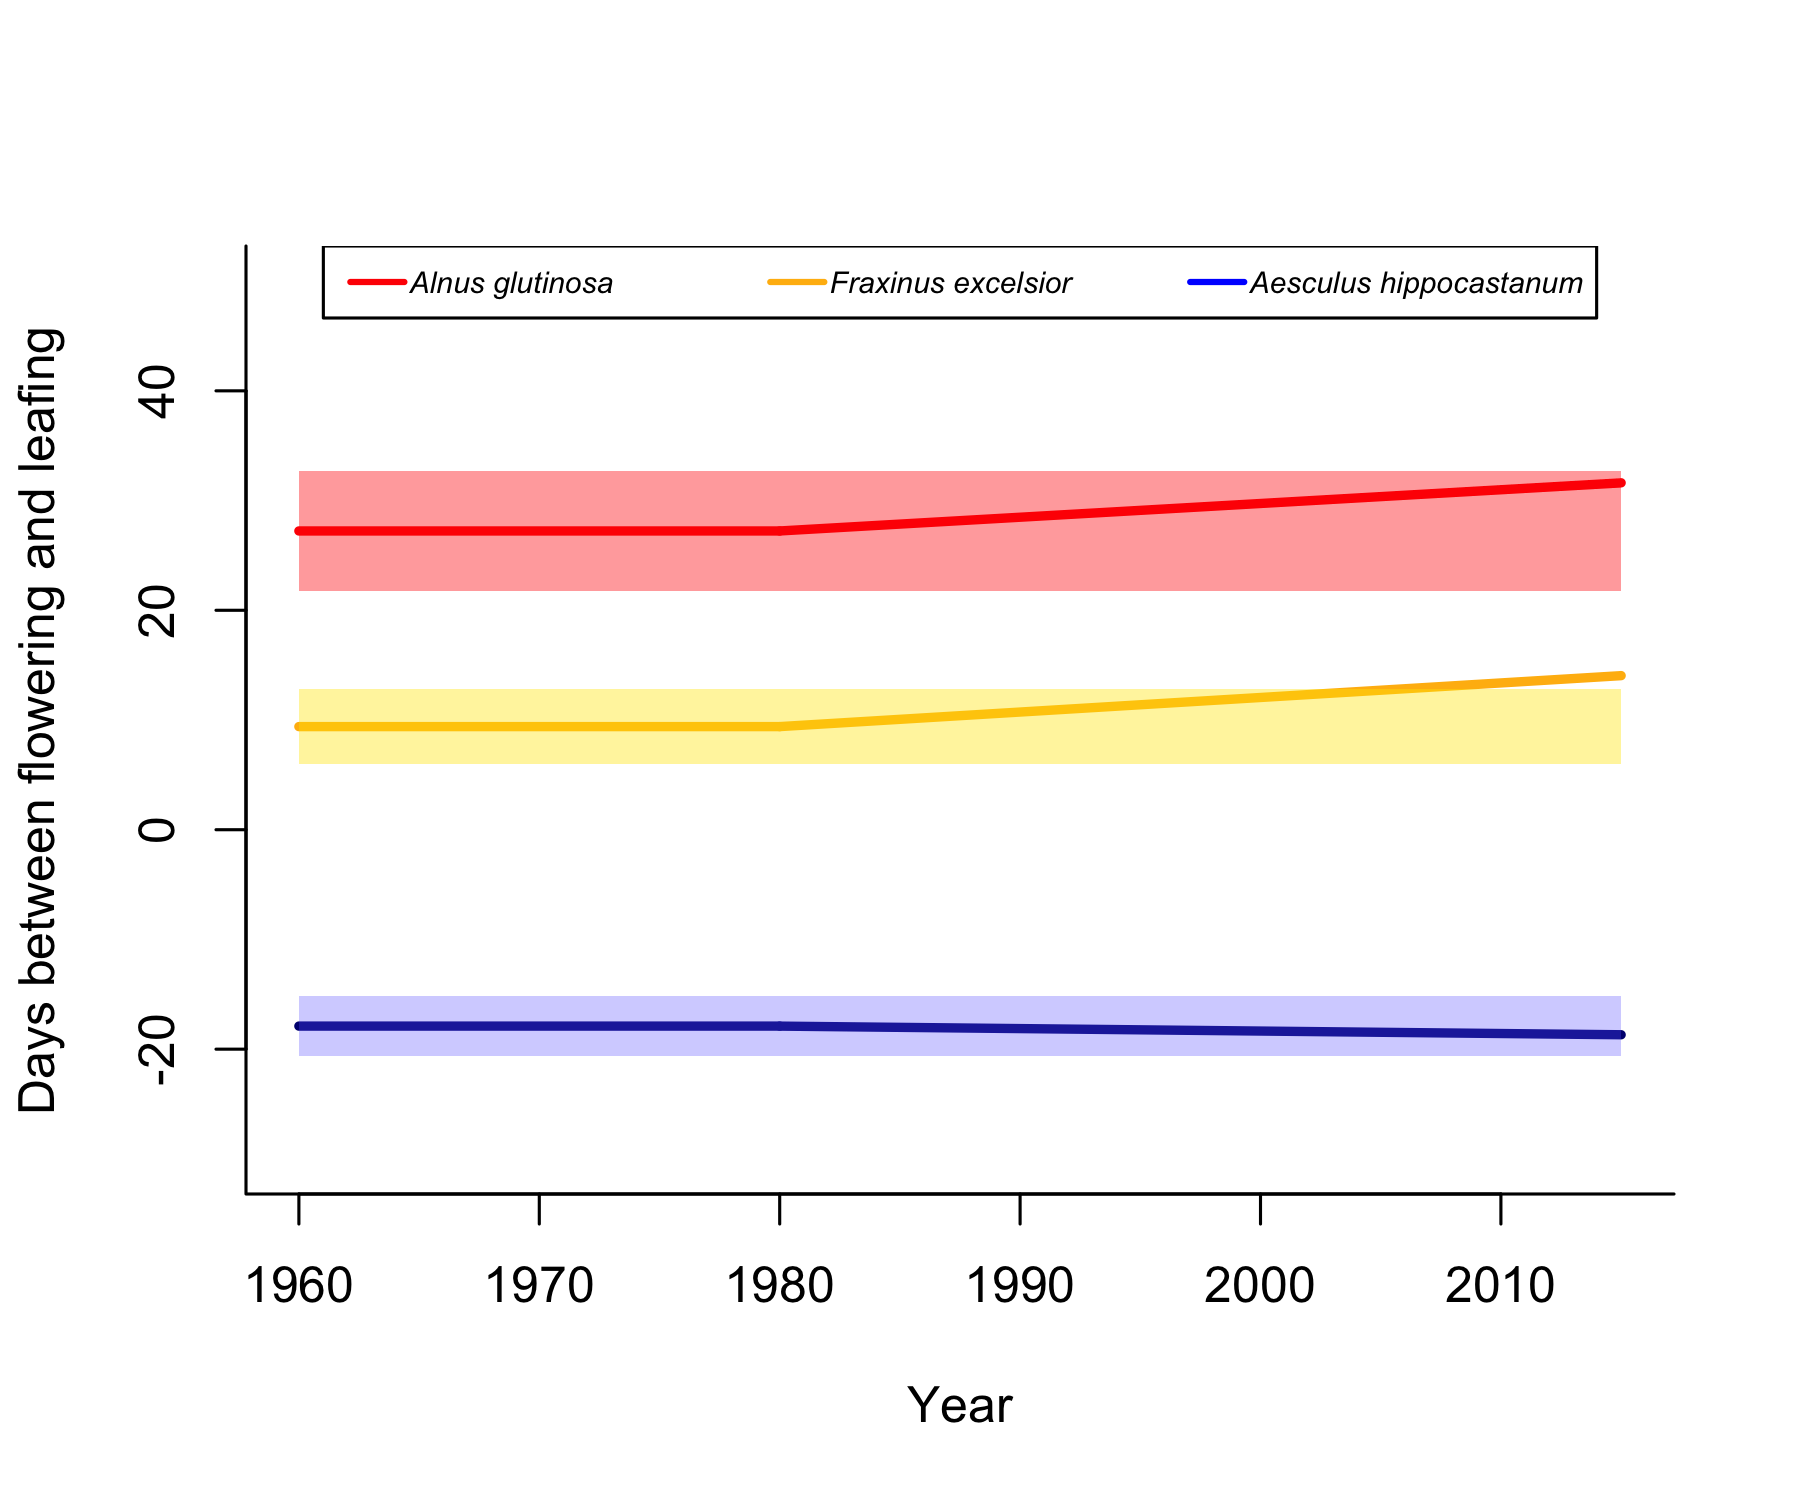
\includegraphics[width=\textwidth]{..//figure/FLS_climate_change.png} 
    \caption{\textbf{Modeled FLS response to climate change across Europe for three tree species from 1960 to 2015.} To detect the effect of climate change on average FLS, the models allows for shifts in FLS after 1980. Each line represents a population from the PEP725 database and the highlighted regions indicate historic range of FLS variability (upper and lower 95\% credible intervals of the pre-1980 average). There is significant intra-specific variation in average FLS and the FLS response to climate change. For all species, the time between flowering and leafing is generally increasing but the direction and rate of change differs across species and sites.}
    \label{fig:Figure 1}
\end{figure}

\begin{figure}[ht]
    \centering
    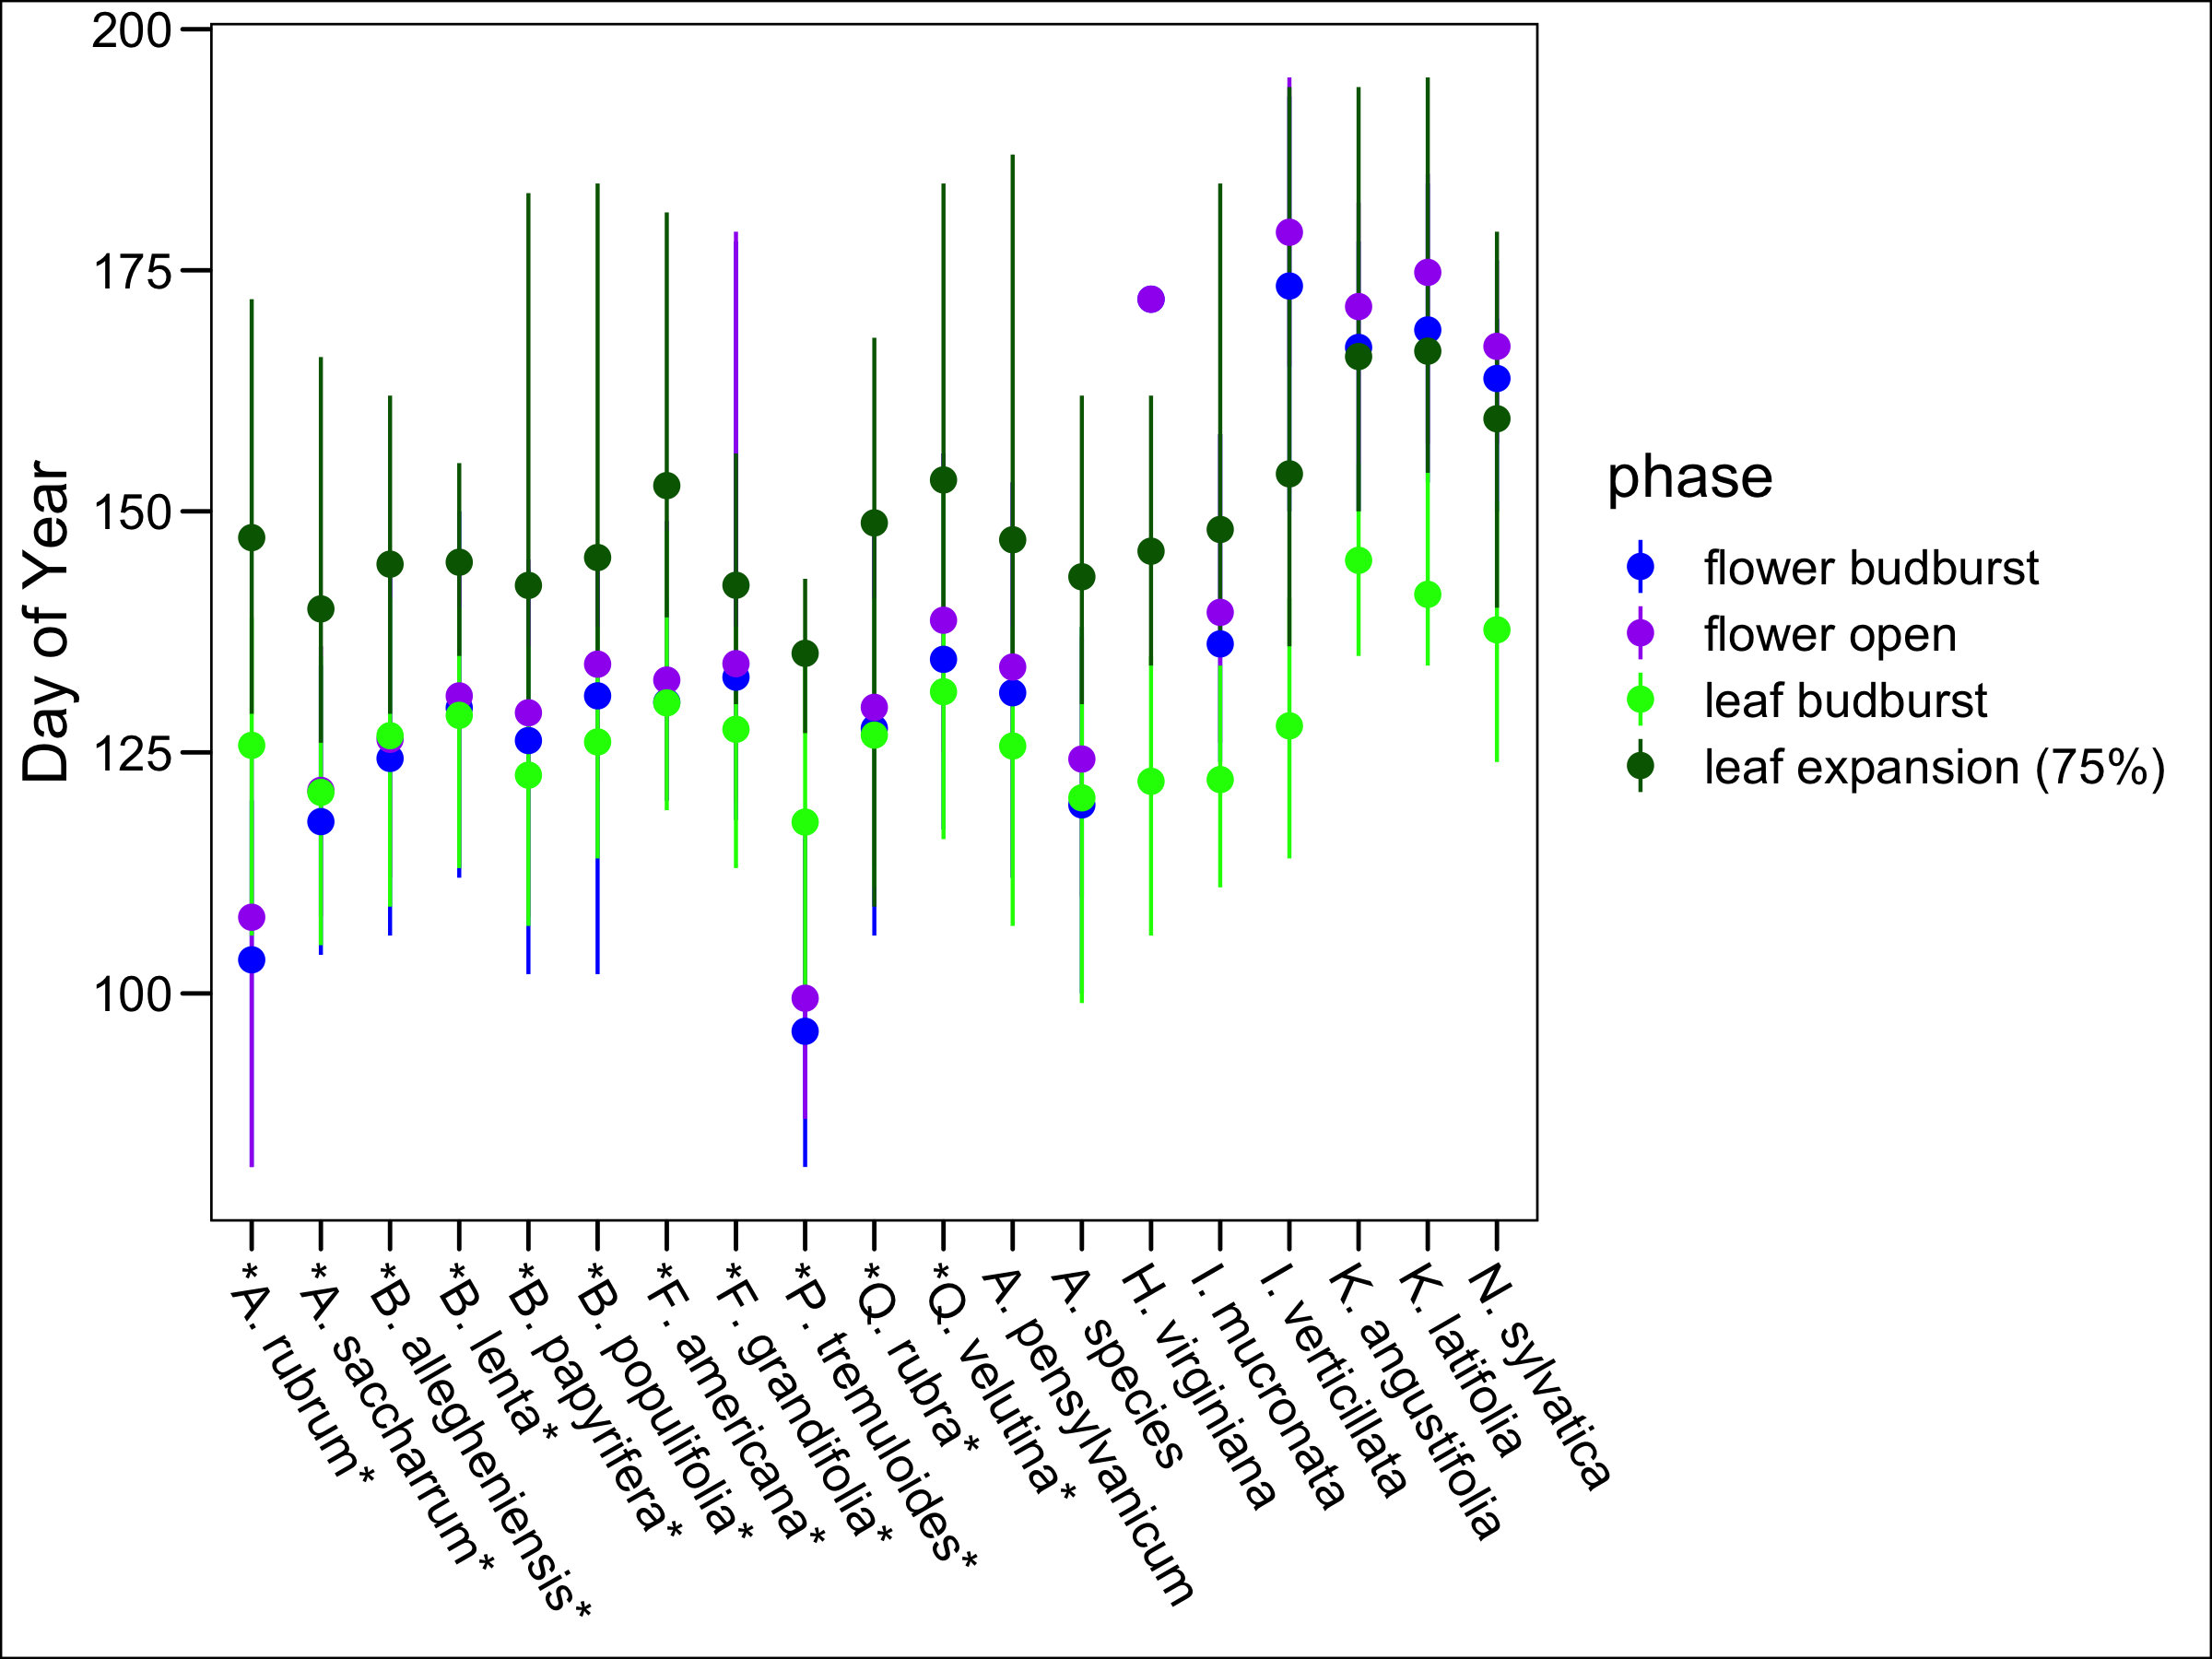
\includegraphics[width=\textwidth]{..//figure/HFmeans_expanded.png}
    \caption{\textbf{Average inter-specific FLS variation at Harvard Forest, MA from 1990-2015.} This community displays all major FLS patterns, but because of overlapping floral and vegetative sub-phases and interannual variability in phenology (lines indicate standard errorfor each phenophase mean), it is difficult to neatly assign all species to a FLS category. Other notable patterns relevant to the FLS hypotheses can be seen. 1) As predicted by the early flowering hypothesis, the earliest species to initiate spring phenology are hysteranthous. 2) As predicted by the pollination syndrome hypothesis, wind-pollinated species (indicated with a *) may vary in whether their flowers or vegetative buds break first, but all open their flowers before leaves expand to 75\%.}
    \label{fig:Figure 2}
\end{figure}

 \begin{figure}[ht]
        \centering
          
\includegraphics[width=\textwidth]{..//figure/HF_Q_ru_interannual.jpeg}
        \caption{\textbf{Individual FLS variability over time for \textit{Quercus rubra} at Harvard Forest.} While this species is typically is classified as synanthous, we see here that the the order of flower and leaf bud break, and the time between these events varies considerably for each individual over time, and between individuals in any given year. None of this variation can be accounted for in a catagorical FLS classification system.}
        \label{fig: Figure 3}
    \end{figure}
  

        \begin{figure}[ht]
    \centering
    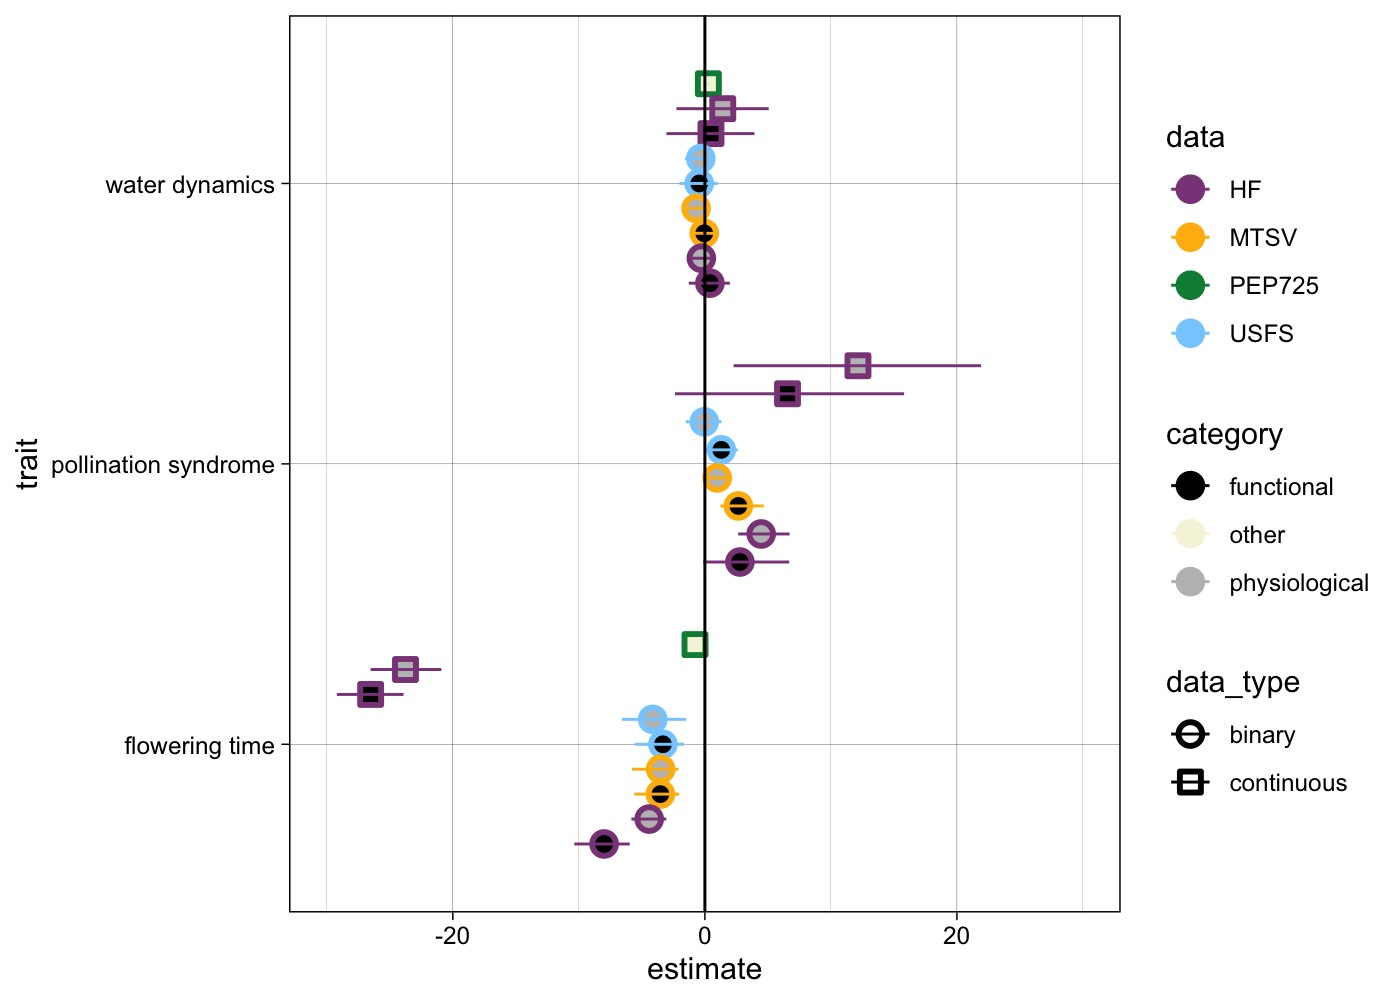
\includegraphics[width=\textwidth]{..//figure/allmods_effectsizes_combined.jpeg}
    \caption{Estimated effects of water dynamics (minimum precipitation across species range or average soil moisture), pollination syndrome, and flowering time on FLS patterns across four case studies. We used phylogenetic adjustments and standardized units to make a basic comparison of four datasets of different taxonomic scopes (intra-vs. interspecific variation) data types (categorical and continuous) and definitions of of FLS. While absolute parameter estimates should not be directly compared due to scaling inconsistencies between models and different modeling approaches for differing data structure, all models support the consensus that wind pollination and early flowering is associated with a flowering first FLS, and there is little effect of measures of water dynamics. Lines represent 95\% bootstrap or credible intervals depending on the modeling framework.}
    \label{fig:Figure 4}
    \end{figure}



\bibliography{..//refs/hyst_outline.bib}



\end{document}

%Several hypotheses, which will be discussed in more detail in the next section, have been put forward \itepAckerman200,Whitehead1967,Franlkin2006, Janzen1967,Primack1987, Gougherty2018, but direct tests of the fitness benefits of this FLS are rare.
%\section*{Case Studies}
%\indent\indent To further explore the current FLS hypotheses and evaluate how the categorization of FLS and intraspecific variation impact their interpretation, we modeled associations between relevant functional and environmental traits and measures of FLS in four datasets from the temperate northern hemisphere. We will begin by introducing each data set, briefly describing the data structure, modeling choices and inference space for each case. We then compare our resulting models for each case study, considering how these four cases in concert both clarify and complicated the FLS hypotheses at the inter- and intraspecific levels. 
%\subsubsection*{Data set I: Michigan Trees; Michigan Shrubs and Vines (MTSV)}
 %\indent\indent The first data set is complied from two regional guides books, Michigan Trees \citep{Barnes} and Michigan Shrubs and Vines \citep{Barnes}, in which FLS for 194 woody plants species of eastern North America are given through qualitative, verbal descriptions. In organizing these descriptors into FLS categories, We applied two alternate categorization schemes. Our \textit{functional} FLS classification was meant to accommodate a degree of overlap between flowering and the early stages of leaf out as predicted by the wind pollination hypothesis. In this system, FLS descriptions of "flowers before leaves", "flowers before/with leaves" and "flowers with leaves" were classified as the flowering first FLS. Our \textit{physiological} classification restricted any overlap for the flowering-first classification, and only species described as "flowers before leaves" were considered as flowering-first.
% \subsubsection*{Data set II: United States Forest Services Silvics Manual Vol. II (USFS)}
 %\indent\indent The second data set was compiled from the United States Forest Service's Silvics Manual Vol II \citep{}. These data consist of FLS description for 81 woody plant species, including species from both the eastern and western United States. For the USFS data, we applied the same FLS classification scheme as describe above for the MTSV data. Because of the similar structure of these two datasets, we can evaluate the influence of the data source on FLS inference by comparing the respective model results.
 %\subsubsection*{Data set III: Phenology of Woody Species at Harvard Forest since 1990 (HF)}
%\indent\indent A third data set, already addressed briefly in previous sections, comes from long term phenological observations at Harvard Forest in Petersham MA \citep{O'keefe}. For this case study, we calculated a quantitative estimate of FLS, "FLS offset", defined as flowering day of year subtracted from the leafing day of year, for 24 of the deciduous species from the HF data. Positive values of FLS offset indicate a flowering first FLS, while negative values indicate a leafing first strategy.
%The phenology data was recorded at the individual tree level, and can therefore be used to address question of FLS at both intra- and Inter-specific level. With these quantitative FLS estimates, we approximated our FLS classifications from the categorical data by defining "physiological offset" as the difference between flower and leaf budburst day, and "functional FLS offset" as the difference between flower open day and the day on which expanding leaves 75\% of full size. With these data, we also evaluated the effect of qualitatively categorizing FLS at the species level directly by collapsing positive values of average FLS offset to "flowering first" and average negative values to "leafing first", and comparing the results to the quantitative models.
%\subsubsection*{Data set IV:  The Pan European Phenology Project (PEP725)}
%\indent\indent For the final case study, we obtained long term flowering and leafout observations for 3-7 flowering-first species across Europe from the Pan European Phenology Project's database \citep{}. These data are temporally and spatially explicit allowing for us to calculate FLS offset at each site/year. We included any observation stations with more than 10 years worth of both flowering and leafing observations. While the data set is species poor, this criteria allows for a robust evaluation of individual and population level variability in FLS.\\

%\indent\indent We used the MTSV,USFS and HF datasets to model species level FLS trait association. For these models, we chose three predictors relevant to the existing FLS hypotheses; pollination syndrome (wind pollination hypothesis), flowering time (early flowering hypothesis) and minimum precipitation tolerance across a species' range (water dynamic hypothesis). We also measured the phylogenetic structure of categorical FLS, based on a published angiosperm phylogeny \citep{Zanne}(phylogenetic conservatism hypothesis). \\
%\indent Our investigation of FLS in the PEP725 data focused on intraspecific FLS variation. We tested the predictions of the "early flowering" and "water dynamics hypothesis", evaluating how the interannual and population level variability in FLS was affect by environmental parameters average soil moisture, average last frost date, and precipitation.  

%\section*{Aggregated evidence for the FLS hypotheses}
%\begin{enumerate}
%    \item In the following section we will discuss how considering the collective results from our case studies affect our understanding of the hypotheses. We find associations between functional traits hysteranthy that are predicted by several hypotheses suggesting support for them. 
 %   \begin{enumerate}
  %      \item But these data are limited.
   %     \item Variation in this traits at the intraspecific level should have clear fitness consequences.
    %    \item For example given the same levels of ambient pollen, individuals with more hysteranthy should capture more pollen.
     %   \item these kinds of data haven't been collected, but would allow for a more directed evaluation of the hypotheses.
      
    %\end{enumerate}
  %\item  Considering fitness more explicitly into the study of hysteranthy would be a way to better test the predictions, and this will be discussed below
%\end{enumerate} 

. %say this way bettern
%\subsubsection*{Wind pollination hypothesis}
%\begin{enumerate}
%    \item The wind pollination hypothesis predicts that hysteranthy should be associated with the wind pollination syndrome, and that intraspecific variation in FLS should be minimal because pollination syndrome is conserved at the species level. 
 %   \item Our three interspecific variability models generally supported this prediction, although the strength of the association varied depending on the FLS categorization scheme.
 %   \item As predicted, functional hysteranthy generally showed a stronger association with pollination syndrome.
%    \item Intra-specific hysteranthy variability was higher than expected, given the hypotheses.  One of two things could be happening.
 %   \begin{enumerate}
  %     \item As we mentioned there is there is probably a thresh hold below which small leaves don't matter. It could be that the variability never crosses this thresh hold.
   %     \item Considering individual variability, pollination success is actually reduced in years where flower-leaf overlap increases, but the variability is maintained through physiological constraints and balancing selection.
    %\end{enumerate}
    %\item There is a reasonable framework for testing these possibilities. 
%    \begin{enumerate}
 %       \item Study have modeled pollen flow through open vs. closed canopies, but these kinds of studies couldb e performed at higher temporal resolution to capture this effect at various stages of leaf expansion.
  %      \item you could monitor trees over multiple season to see if variation in hysteranthy correlates with variation in pollination success, or directly manipulate hysteranthy in controlled environments.
   % \end{enumerate}
    %\item Even with this general support of the wind pollination hypothesis, there are a nontrivial number of hysteranthous biotically pollinated taxa. Surely, wind pollination can't explain hysteranthy in these species. Exploring trait associations in this taxonomic subset may help clarify the importance of the other hypotheses.  
    %\end{enumerate}

%\subsubsection*{Water dynamics}
%\begin{enumerate}
 %   \item This water dynamics hypothesis suggests that hysteranthous flowering is drought tolerance adaptation. At the species level, it predicts that increased drought tolerance should be associated with hysteranthous flowering. At the intraspecific level, populations growing in drier regions should show more pronounced hysteranthy and even that hysteranthous offset would increase in dry vs. wet years.
  %  \item We found little support for this hypothesis in our analysis.
   % \begin{enumerate}
    %    \item No effect of drought tolerance in any of the the interspecific models specific.
     %   \item At the intraspecific level, we found that drought years were actually associated with reduced hysteranthy due to a delay in flower.
     %   \item There was a week effect of lower soil moisture predicting increased hysteranthy at the population level when considered alone, but this effect flipped directions when other predictors of hysteranthy, such as early flowering were included in the model. Probably need to explain this more.%
    %\end{enumerate}
    %\item This is surprising given that a recent study using a subset of our data found support for this hypothesis. 
%    \begin{enumerate}
 %       \item This could because because the available trait (min P across range) is not a good proxy for drought tolerance.
 %       \item Or, it could be that water in temperate zone isn't usually limited in the spring, and any species level variation due to drought tolerance arose deeper in evolutionary history. If this is the case, more explicitly incorperating biogeopgraphy into our analysis could help us understand this hypothesis.
  %      \item You could also more explicitly test the predictions of this hypothesis, by investigating the intra-specific FLS variation in long term drought experiments.
   % \end{enumerate}
%\end{enumerate}
%\subsubsection*{Early flowering hypothesis}
%\begin{enumerate}
 %   \item This hypothesis predicts that hysteranthy should be associated with the earliest flowering species. At the species level, it would also suggest that there may be associations between hysteranthy and other functional traits associated with early flowering. At the intraspecific level, this hypothesis predicts that years in which flowering occurs early should be associated with increased hysteranthy. Note*, does it make prediction about populations?
  %  \item All of our analyses should strong support for this hypothesis.
   % \item In all three interspecific models, early flowering time was the strongest predictor of hysternathy no matter how hysteranthy was classified. This effect was maintained even we when subset our data to include only generally early flowering species. See supplement.
  %  \item We also found a strong associated between early flowering and hysteranthous offset at the intraspecific level as well.
  %  Early flowering was associated with increase offset, and this relationship was much stronger than the assoication between early leafing and hysteranthy offset (R2 0.5 vs. 0.03).
   % \item This begs the question does hysteranthy actually matter, or can it be lumped in with the general study of evolution of reproductive phenology, because all that really matters is the absolute timing of flowering and hysteanthy is a physiological by product.
%\item We feel because of the evidence of the wind pollination hypothesis and that relies more on the relative timing of flowering vs leaves as opposed to the absolute timing of one or the other, it is too early to abandon the idea that hysteranthy is a trait of its own.
%\end{enumerate}
%\subsubsection*{Phylogeny}
%\begin{enumerate}
 %   \item This hypothesis predicted that interspecific variation in hysteranthy should show strong phylogenetic patterning in lieu of other functional trait associations. There were no clear prediction about intraspecific variation that could be made without a better understanding of the genetic structure of the populations we examined, so for this hypothesis, we restrict our analysis to hysteranthy at the interspecific level.
  %  \item The phylogenetic signal of hysteranthy, as measured by a D statistics when hysteranthy was treated as a categorical trait and by pagaels lambda when hysteranthy was treated continuous, varied significantly between data sources, and depended on how hysteranthy was classfied.
  %  \item This is not surprising.
   % \begin{enumerate}
    %    \item Changing the classification scheme dramatically changed the patterning of the trait along the tree. See supplement.
     %   \item Also it would be expected that except under extremely high phylogenetic structure changing the number and identities of species in the tree would change the inference.
      %  \item Also, several of the hypotheses (wind pollination, early flowering) correspond to traits that have been show to have their own high phylogenetic structure. *Need another sentence about this.
       % \item Overall, the phylogenetic structure of hysteranthy is low-intermediate. *Might need help about how to say something about this that is a bit smarter.
  %  \end{enumerate}
    
%\subsection*{Hysteranthy and global change}
%Above, we recommended that several of the hysteranthy hypotheses could be better tested be relating variability in hysteranthy to explicitly to fitness measures. This approach is also essential in the context of global change. We began this paper by suggesting FLS patterns are changing with global climate change. IF we can better understand the role of this change in overall plant fitness, will better be able to predict the plant communities of the future and implement conservation and natural resource policies accordingly.
%\end{enumerate}
 %\begin{figure}
  %  \centering
   % 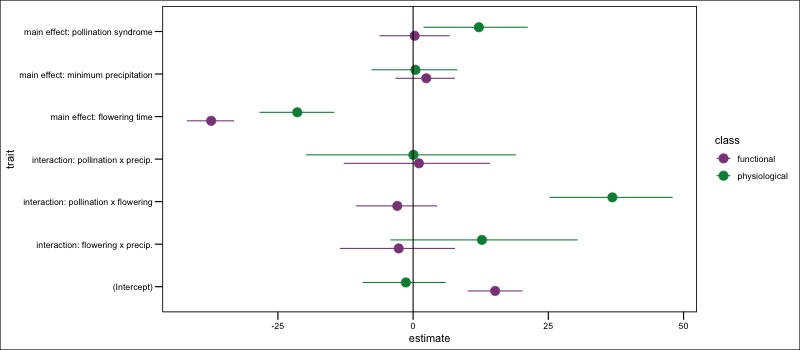
\includegraphics[width=\textwidth]{..//figure/HF_cont_effectsize.jpeg}
    %\caption{Harvard forest continuous . Estimates, 95\% bootstrapping intervals depicted}
    %\label{fig:Figure 6}
    %\end{figure}

%   \begin{figure}[h!]
    %\centering
    %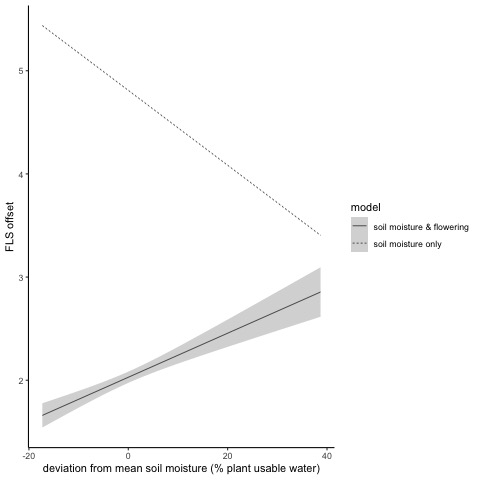
\includegraphics[width=\textwidth]{..//figure/SM_comp.jpeg}
    %\caption{effect of soil moisture on FLS offset with (dashed) and without (solid) considering flowering time}
    %\label{fig:Figure 5}
    %\end{figure}
%Long Abstact:
%\indent\indent As the study of phenology progresses as a discipline, it is increasing clear that it is not only individual phenological events that affect organism fitness and ecological functioning, but also the relationship between stages. Deciduous woody plants exhibit considerable variation in the relative order of their reproductive and vegetative events, or their flower-leaf  sequence (FLS). A century of research suggests that FLS patterns are adaptive, and several competing hypotheses stand to explain their evolution and function. \\
%\indent Reconciling these hypotheses has been impeded by our conceptual orientation towards them. Classically, FLSs are treated as discrete categories and described at the species level. However, this framework obscures important inter-specific differences and masks substantial intra-specific variation ignored by the hypotheses. Here, we review and modify the existing hypotheses to account for the high levels of both inter- and intra-specific FLS variation seen in nature. We then evaluate these hypotheses with four case studies from temperate forest species.\\ 
 %\indent Our review and case studies provide three major insights towards a new conceptual framework for understanding FLSs. First, we find concurrent support for multiple hypotheses. Future research should accommodate this coincidence by allowing for overlapping hypotheses in large community models and by testing individual hypotheses in smaller sub-groupings that control for variation in other traits. Second, we show that the support for FLS hypotheses is highly sensitive to how FLSs are defined. Researchers should, when possible, move away from the classic categorization scheme and use continuous measures of FLS, such as number of days between flowering and leafing. Finally, researchers should use these intra-specific, continuous data to test for fitness consequences in FLS variation. This will advance our understanding of the fundamental biology of FLSs, and help us to predict how climate-related alterations to FLSs will affect tree communities in the changing future.
